%% IEEE conference paper (English)
%% Compile:  pdflatex SaraBabic_paper && bibtex SaraBabic_paper && pdflatex SaraBabic_paper && pdflatex SaraBabic_paper
\documentclass[conference]{IEEEtran}
\IEEEoverridecommandlockouts

\usepackage[T1]{fontenc}
\usepackage[utf8]{inputenc}
\usepackage{lmodern}
\usepackage{cite}
\usepackage{amsmath,amssymb}
\usepackage{graphicx}
\usepackage{booktabs}
\usepackage{url}
\usepackage{microtype}
\usepackage{xcolor}

\begin{document}

\title{Does Social Interaction Modeling Actually Help?\\
A Controlled Comparison of Graph-Based and\\
Interaction-Agnostic Pedestrian Trajectory Prediction}

\author{\IEEEauthorblockN{Sara Babić}
\IEEEauthorblockA{\textit{Machine Learning and Artificial Intelligence} \\
\textit{Faculty of Technical Sciences, University of Novi Sad}\\
Novi Sad, Serbia}}

\maketitle

\begin{abstract}
Socially-aware robot navigation requires predicting where nearby pedestrians will be
several seconds into the future. The dominant assumption in this literature is that
explicitly modeling social interaction, typically through graph neural networks or
attention, is the key ingredient for accurate prediction. We show that on the standard
ETH-UCY benchmark this assumption is not supported once the comparison is properly
controlled. We implement three models under an identical data pipeline and evaluation
protocol: a vanilla LSTM baseline trained with an $L_2$ objective, the graph-based
Social-STGCNN trained with a bivariate Gaussian negative log-likelihood, and, as a
control, the same LSTM equipped with an identical probabilistic head and loss. The
conventional comparison between the first two models is confounded, since they differ
simultaneously in architecture and in training objective. When only the architecture
differs, the interaction-agnostic model attains an average displacement error of
$0.405$~m against $0.415$~m for the graph model, i.e. no measurable advantage from social
modeling; the graph model wins on only one of five scenes. Both models reproduce
published performance, confirming that this is a property of the benchmark rather than of
the implementation. What does yield a substantial improvement is uncertainty modeling
($0.552 \rightarrow 0.405$~m, a $27\%$ reduction), obtained by predicting a distribution
instead of a point, and parameter efficiency: the graph model matches the LSTM using
$7{,}563$ versus $199{,}106$ parameters, a $26\times$ reduction. We additionally describe
a block-diagonal graph batching scheme that accelerates graph training by $24\times$. Our
results suggest that for socially-aware navigation the practically valuable output is a
calibrated distribution over future positions rather than a structured interaction model.
\end{abstract}

\begin{IEEEkeywords}
trajectory prediction, socially-aware navigation, graph neural networks, LSTM,
uncertainty estimation, ETH-UCY, controlled comparison
\end{IEEEkeywords}

\section{Introduction}

A robot sharing space with people cannot treat them as static obstacles. Classical
planners such as A*, RRT or DWA optimize path length or traversal time against a snapshot
of the environment, and consequently produce manoeuvres that are collision-free yet
socially unacceptable: cutting through a conversing group, passing uncomfortably close, or
freezing in place when every direction appears blocked, the well-known \emph{freezing
robot problem}~\cite{trautman2010unfreezing}. Making a planner socially aware therefore
requires a perception layer that answers a predictive question: where will each person be
several seconds from now, and with what confidence~\cite{mavrogiannis2023core}?

This has motivated a large body of work on pedestrian trajectory prediction, and a clear
methodological trend within it. Since Social-LSTM~\cite{alahi2016social} introduced social
pooling, successive architectures have modeled inter-agent interaction ever more
explicitly - through generative modeling~\cite{gupta2018social}, graph
convolution~\cite{mohamed2020social}, or heterogeneous graph
structures~\cite{salzmann2020trajectron}. The implicit premise is that interaction
modeling is where predictive accuracy comes from.

This paper questions that premise, not by proposing yet another architecture, but by
constructing a comparison that isolates it. Our starting observation is that the usual
comparison in this literature is confounded. An interaction-agnostic baseline is typically
trained with a deterministic $L_2$ objective, whereas the proposed social model is
probabilistic and trained with a negative log-likelihood, then evaluated under a
best-of-$K$ sampling protocol. The two models therefore differ in \emph{two} variables
simultaneously - architecture and training objective - and any observed difference cannot
be attributed to social modeling alone.

We remove the confound by introducing a third model: the same interaction-agnostic LSTM,
given an identical bivariate Gaussian head, trained with the identical loss, selected by
the identical criterion, and evaluated under the identical protocol as the graph model.
Only the architecture then differs.

Our contributions are:

\begin{itemize}
\item A controlled experiment showing that on ETH-UCY, at the standard $4.8$~s horizon,
      graph-based social modeling yields no average accuracy advantage over an
      interaction-agnostic architecture ($0.415$~m vs.\ $0.405$~m ADE).
\item An attribution of where the improvement actually comes from: uncertainty modeling
      reduces ADE by $27\%$, and the graph architecture delivers a $26\times$ reduction in
      parameter count at equal accuracy.
\item A block-diagonal graph batching scheme that makes spatio-temporal graph training
      $24\times$ faster without altering graph propagation.
\item A complete, reproducible implementation in which all three models share one data
      pipeline and one evaluation module, so that no measured difference can originate
      from the data or the metric code.
\end{itemize}

\section{Related Work}

\textbf{Hand-crafted interaction models.} The Social Force model~\cite{helbing1995social}
represented pedestrians as particles subject to attractive and repulsive potentials. Such
models are interpretable but require manual parameter tuning and generalize poorly across
environments.

\textbf{Recurrent models.} Social-LSTM~\cite{alahi2016social} paired a per-pedestrian LSTM
with a social pooling layer aggregating hidden states of spatial neighbours.
Social-GAN~\cite{gupta2018social} introduced adversarial training to produce multiple
socially plausible futures, and established the best-of-$K$ evaluation protocol that
subsequent probabilistic work adopted.

\textbf{Graph-based models.} Social-STGCNN~\cite{mohamed2020social} replaced pooling with
an explicit graph in which nodes are pedestrians and edge weights encode spatial
proximity, combining graph convolution~\cite{kipf2017semi} with temporal convolution in
the spirit of spatio-temporal graph networks for traffic
forecasting~\cite{yu2018spatio}. Trajectron++~\cite{salzmann2020trajectron} extended this
to heterogeneous agents and dynamic constraints.

\textbf{Critical evaluations.} Schöller \textit{et al.}~\cite{scholler2020constant} showed
that a constant velocity model outperforms many published social architectures on ETH-UCY,
arguing that benchmark performance is dominated by individual motion inertia. Our work is
complementary: rather than comparing learned models against a non-learned baseline, we
compare two learned models that are matched in every respect except the presence of
interaction modeling.

\section{Problem Formulation and Dataset}

\subsection{Problem statement}

For pedestrian $i$ we observe a history of positions
$X_i = \{(x_i^t, y_i^t)\}_{t=1}^{T_{obs}}$ and predict the future
$\hat{Y}_i = \{(\hat{x}_i^t, \hat{y}_i^t)\}_{t=T_{obs}+1}^{T_{obs}+T_{pred}}$.
Following standard practice we set $T_{obs} = 8$ and $T_{pred} = 12$. At the $2.5$~Hz
recording rate of the benchmark this corresponds to observing $3.2$~s and predicting
$4.8$~s.

\subsection{Dataset}

We use ETH-UCY~\cite{pellegrini2009you,lerner2007crowds}, comprising five scenes recorded
from a bird's-eye view with positions expressed in world coordinates in metres. Metric
coordinates make the error measures directly interpretable as physical distances, which is
precisely what a planner requires.

Evaluation follows the \emph{leave-one-scene-out} protocol: for each scene, models are
trained on the remaining four and tested on the held-out scene. This measures
generalization to an entirely new physical space rather than to new pedestrians in a
familiar one, which is the realistic condition for a robot entering an unmapped environment. We
adopt the standardized split distributed with~\cite{mohamed2020social}, identical to that
of~\cite{gupta2018social}, so that our numbers are directly comparable to published
results. Table~\ref{tab:dataset} reports the resulting statistics.

\begin{table}[t]
\caption{Dataset statistics under the leave-one-scene-out protocol. A \emph{sequence} is
one 20-frame window; a \emph{trajectory} is one pedestrian present in all 20 frames of
that window.}
\label{tab:dataset}
\centering
\small
\begin{tabular}{lrrrrrr}
\toprule
 & \multicolumn{2}{c}{Train} & \multicolumn{2}{c}{Validation} & \multicolumn{2}{c}{Test} \\
\cmidrule(lr){2-3}\cmidrule(lr){4-5}\cmidrule(lr){6-7}
Scene & Seq. & Traj. & Seq. & Traj. & Seq. & Traj. \\
\midrule
ETH   & 3{,}283 & 30{,}307 & 733 & 5{,}422 & 253 & 364 \\
HOTEL & 3{,}118 & 29{,}676 & 688 & 5{,}203 & 445 & 1{,}197 \\
UNIV  & 2{,}719 & 9{,}874  & 622 & 2{,}800 & 947 & 24{,}334 \\
ZARA1 & 2{,}889 & 28{,}577 & 671 & 5{,}184 & 705 & 2{,}356 \\
ZARA2 & 2{,}681 & 26{,}076 & 590 & 4{,}262 & 998 & 5{,}910 \\
\bottomrule
\end{tabular}
\end{table}

The asymmetry in Table~\ref{tab:dataset} is a direct consequence of the protocol: UNIV is
a dense scene, so holding it out both removes the densest training examples and produces a
test set averaging $25.7$ pedestrians per window, against $1.4$ for ETH.

\section{Methodology}

\subsection{Preprocessing}

A sliding window of $T_{obs}+T_{pred}=20$ consecutive frames traverses each recording.
Within a window we retain only pedestrians present in all $20$ frames, matching the
reference protocol and avoiding padding semantics that would differ from published work.

Crucially, the models operate on \emph{relative displacements}
$\Delta p^t = p^t - p^{t-1}$ rather than absolute coordinates. Each scene has its own
coordinate frame, so a model consuming absolute positions learns where people stand in the
training scenes, which is worthless information in an unseen scene. Displacements make the
model translation invariant, so that it learns how people move. Predicted displacements
are converted back to positions by cumulative summation from the last observed point.

Because scenes contain variable numbers of pedestrians, all pedestrians in a batch are
concatenated along a single dimension while a companion tensor records per-scene
boundaries. The LSTM ignores these boundaries entirely; the graph model uses them to
determine which pedestrians belong to the same graph. A single loader therefore serves all
three models, guaranteeing that they observe byte-identical data.

\subsection{Baseline: vanilla LSTM}

The baseline is an encoder--decoder LSTM~\cite{hochreiter1997long}. A linear layer embeds
each displacement into a $64$-dimensional space; an encoder LSTM with $128$ hidden units
compresses the observed motion into a hidden state; a decoder LSTM autoregressively emits
$12$ future displacements, feeding each output back as the next input. No pedestrian ever
observes another, which is precisely the point, as this isolates how much of the task is
explained by an agent's own inertia. The model has $199{,}106$ parameters and is trained
with the mean Euclidean error over displacements, a quantity directly aligned with the
reported metric. Gradients are clipped to unit norm, as the autoregressive decoder
propagates through twelve chained steps.

\subsection{Graph model: Social-STGCNN}

Social-STGCNN~\cite{mohamed2020social} represents each timestep as a graph whose nodes are
pedestrians. Edge weights are inverse distances,
$a_{ij} = \lVert p_i - p_j \rVert_2^{-1}$, so that nearby pedestrians influence one another
more strongly, a direct formalization of personal space. The adjacency matrix is
symmetrically normalized following~\cite{kipf2017semi},
\begin{equation}
\hat{A} = D^{-1/2}\,(A + I)\,D^{-1/2},
\end{equation}
where the added identity provides self-loops so that a node retains its own features
during aggregation.

We note one deliberate deviation from the reference implementation
of~\cite{mohamed2020social}, which normalizes the adjacency matrix using the normalized
graph Laplacian $L = I - D^{-1/2} A D^{-1/2}$ rather than the normalized adjacency
$\hat{A}$ used here. Since $L = I - \hat{A}$, the two operators differ, and our reported
figures correspond to the formulation above. We adopt $\hat{A}$ because it is the
standard GCN propagation rule~\cite{kipf2017semi}; our results reproduce the published
performance of the original model, so the choice is not detrimental.

Each ST-GCNN block applies a spatial graph convolution followed by a temporal convolution
along the time axis. A Time-Extrapolator CNN then maps the $8$ observed steps to $12$
predicted steps by convolving over the temporal dimension, producing all future steps in a
single pass rather than recurrently.

The output at each step consists of the five parameters of a bivariate Gaussian,
$(\mu_x, \mu_y, \sigma_x, \sigma_y, \rho)$, trained by minimizing the negative
log-likelihood of the observed displacement. Numerical stability is enforced by
parameterizing $\sigma = \exp(\cdot)$ and $\rho = \tanh(\cdot)$ with clamping, without
which NLL training diverges in practice. The model has only $7{,}563$ parameters.

\subsection{Controlled comparison: probabilistic LSTM}

The two models above differ in architecture \emph{and} in training objective. A model
trained with NLL has a mean that is not optimized for $L_2$ error, so evaluating that mean
against an $L_2$-trained baseline penalizes the graph model for reasons unrelated to
social modeling. Conversely, comparing best-of-$20$ sampling against a single deterministic
prediction compares twenty attempts with one. Neither comparison answers the question of
interest.

We therefore introduce a control: the same vanilla LSTM, with its output head widened from
two to five values, trained with the \emph{identical} bivariate NLL loss, selected on the
\emph{identical} validation criterion, and evaluated under the \emph{identical}
best-of-$20$ protocol as the graph model. The loss function and sampling routine are
literally the same code paths, so the protocols cannot silently diverge. The two models
now differ in exactly one respect: whether the architecture can observe other pedestrians.

\subsection{Efficient batched graph training}
\label{sec:blockdiag}

A direct implementation processes one scene per optimizer step, as in the reference
implementation. With $3{,}283$ sequences per epoch this issues thousands of very small GPU
launches. Profiling the ETH training loop attributes $0.2$~s per epoch to data loading,
$9.0$~s to adjacency construction and $34.1$~s to the forward and backward passes, for
approximately $62$~s per epoch including validation, or about $13$~hours for all five scenes.

We instead pack $B$ scenes into a single graph whose adjacency matrix is block diagonal.
Pedestrians from different scenes have no edge between them, so graph propagation is
identical to processing the scenes separately, while the computation is issued as one GPU
call. Combined with vectorized best-of-$K$ sampling and periodic rather than per-epoch
validation, this reduces training to $2.6$~s per epoch, a $24\times$ speedup; all five
scenes train in roughly $15$~minutes.

We note for completeness that batch normalization now computes statistics over all nodes
in the batch rather than over a single scene. This is standard mini-batch behaviour and
generally stabilizes training, but it is not a bit-identical computation.

\subsection{Hyperparameter optimization}

Architecture and learning rate are selected using Optuna~\cite{akiba2019optuna} with a
Tree-structured Parzen Estimator sampler~\cite{bergstra2011algorithms} and median pruning.
The search space covers learning rate, the number of graph convolution blocks, the depth of
the temporal decoder, the temporal kernel size and dropout. The objective is
\emph{validation} ADE; the test set is never consulted during the search, as selecting
hyperparameters on test performance constitutes information leakage that silently inflates
reported results.

\section{Experimental Setup}

\subsection{Metrics}

We report the two standard measures. Average Displacement Error is the mean
\emph{Euclidean} distance between predicted and true positions over all predicted steps and
all pedestrians,
\begin{equation}
\mathrm{ADE} = \frac{1}{N\,T_{pred}}\sum_{i=1}^{N}\sum_{t=T_{obs}+1}^{T_{obs}+T_{pred}}
\left\lVert \hat{p}_i^{\,t} - p_i^{\,t} \right\rVert_2 ,
\end{equation}
and Final Displacement Error is the distance at the final predicted step,
\begin{equation}
\mathrm{FDE} = \frac{1}{N}\sum_{i=1}^{N}
\left\lVert \hat{p}_i^{\,T_{obs}+T_{pred}} - p_i^{\,T_{obs}+T_{pred}} \right\rVert_2 .
\end{equation}
Both are expressed in metres. Errors are accumulated as sums over pedestrians and divided
once at the end, since averaging per-batch means would misweight batches containing
different numbers of pedestrians.

\subsection{Protocols}

For probabilistic models we report both a \emph{deterministic} figure, obtained from the
mean of the predicted distribution, and the \emph{best-of-20} figure standard in the
literature, in which $20$ trajectories are sampled and the per-pedestrian minimum is
retained. Reporting only one of the two would mislead in opposite directions.

\subsection{Implementation}

All models are implemented in PyTorch and trained with Adam on a single NVIDIA RTX 4050
laptop GPU. The deterministic LSTM baseline is trained for $100$ epochs; the probabilistic LSTM and
Social-STGCNN are both trained for $250$ epochs, so that the two models entering the
controlled comparison receive an identical training budget. Checkpoints are selected by
validation ADE in every case. The complete pipeline (three models, hyperparameter search
and figures) runs in approximately $65$ minutes.

\section{Results}

\subsection{Validation against published results}

Table~\ref{tab:published} compares our models against published figures. Both fall within
the published range; Social-STGCNN in fact surpasses its published average and its
per-scene results on HOTEL, UNIV and ZARA2. This confirms that the protocol and evaluation
are implemented correctly, which is the precondition for trusting the comparisons that
follow.

\begin{table*}[t]
\caption{Comparison with published results (average ADE / FDE over the five scenes, in
metres) and parameter counts.}
\label{tab:published}
\centering
\small
\begin{tabular}{lccr}
\toprule
Model & Ours & Published & Params \\
\midrule
LSTM baseline (det.)        & 0.552 / 1.159 & 0.70 / 1.63~\cite{gupta2018social} & 199{,}106 \\
LSTM-prob (best-of-20)      & 0.405 / 0.761 & n/a                                & 199{,}493 \\
Social-STGCNN (best-of-20)  & 0.415 / 0.784 & 0.44 / 0.75~\cite{mohamed2020social} & \textbf{7{,}563} \\
\bottomrule
\end{tabular}
\end{table*}

\subsection{The confounded comparison}

Table~\ref{tab:deterministic} presents the comparison as it is conventionally made,
between the $L_2$-trained baseline and the deterministic output of the graph model. The
graph model is marginally \emph{worse} on average ($0.563$ vs.\ $0.552$~m). As argued in
Section~IV-D, this comparison is confounded by the difference in training objective and
should not be read as evidence about social modeling.

\begin{table}[t]
\caption{Confounded comparison: deterministic predictions from models trained with
different objectives ($L_2$ vs.\ NLL). ADE / FDE in metres; lower is better.}
\label{tab:deterministic}
\centering
\small
\begin{tabular}{lcc}
\toprule
Scene & LSTM ($L_2$) & Social-STGCNN (NLL mean) \\
\midrule
ETH   & \textbf{1.007} / \textbf{1.996} & 1.043 / 2.113 \\
HOTEL & 0.457 / 0.936 & \textbf{0.436} / \textbf{0.880} \\
UNIV  & 0.577 / 1.278 & \textbf{0.568} / \textbf{1.202} \\
ZARA1 & \textbf{0.402} / \textbf{0.886} & 0.419 / 0.904 \\
ZARA2 & \textbf{0.316} / \textbf{0.699} & 0.350 / 0.761 \\
\midrule
Average & \textbf{0.552} / \textbf{1.159} & 0.563 / 1.172 \\
\bottomrule
\end{tabular}
\end{table}

\subsection{The controlled comparison}

Table~\ref{tab:controlled} contains the paper's central result. Both models now share an
identical probabilistic head, loss function, selection criterion and evaluation protocol;
the only difference is whether the architecture observes other pedestrians.

\begin{table}[t]
\caption{\textbf{Controlled comparison.} Both models use an identical bivariate Gaussian
head, NLL loss and best-of-20 protocol; only the architecture differs: LSTM-prob never
observes other agents, Social-STGCNN does. ADE / FDE in metres; lower is better.}
\label{tab:controlled}
\centering
\small
\begin{tabular}{lcc}
\toprule
Scene & LSTM-prob & Social-STGCNN \\
\midrule
ETH   & \textbf{0.775} / \textbf{1.405} & 0.819 / 1.582 \\
HOTEL & 0.342 / 0.659 & \textbf{0.311} / \textbf{0.561} \\
UNIV  & \textbf{0.411} / 0.816 & 0.412 / \textbf{0.803} \\
ZARA1 & \textbf{0.276} / \textbf{0.497} & 0.283 / 0.498 \\
ZARA2 & \textbf{0.221} / \textbf{0.428} & 0.251 / 0.474 \\
\midrule
Average & \textbf{0.405} / \textbf{0.761} & 0.415 / 0.784 \\
\bottomrule
\end{tabular}
\end{table}

The interaction-agnostic model attains a better average ADE than the graph model
($0.405$ vs.\ $0.415$~m). Social-STGCNN wins on only one scene, HOTEL; it loses on the
remaining four. Fig.~\ref{fig:curves} shows that the two models
also converge to indistinguishable validation error during training.

\begin{figure}[t]
\centering
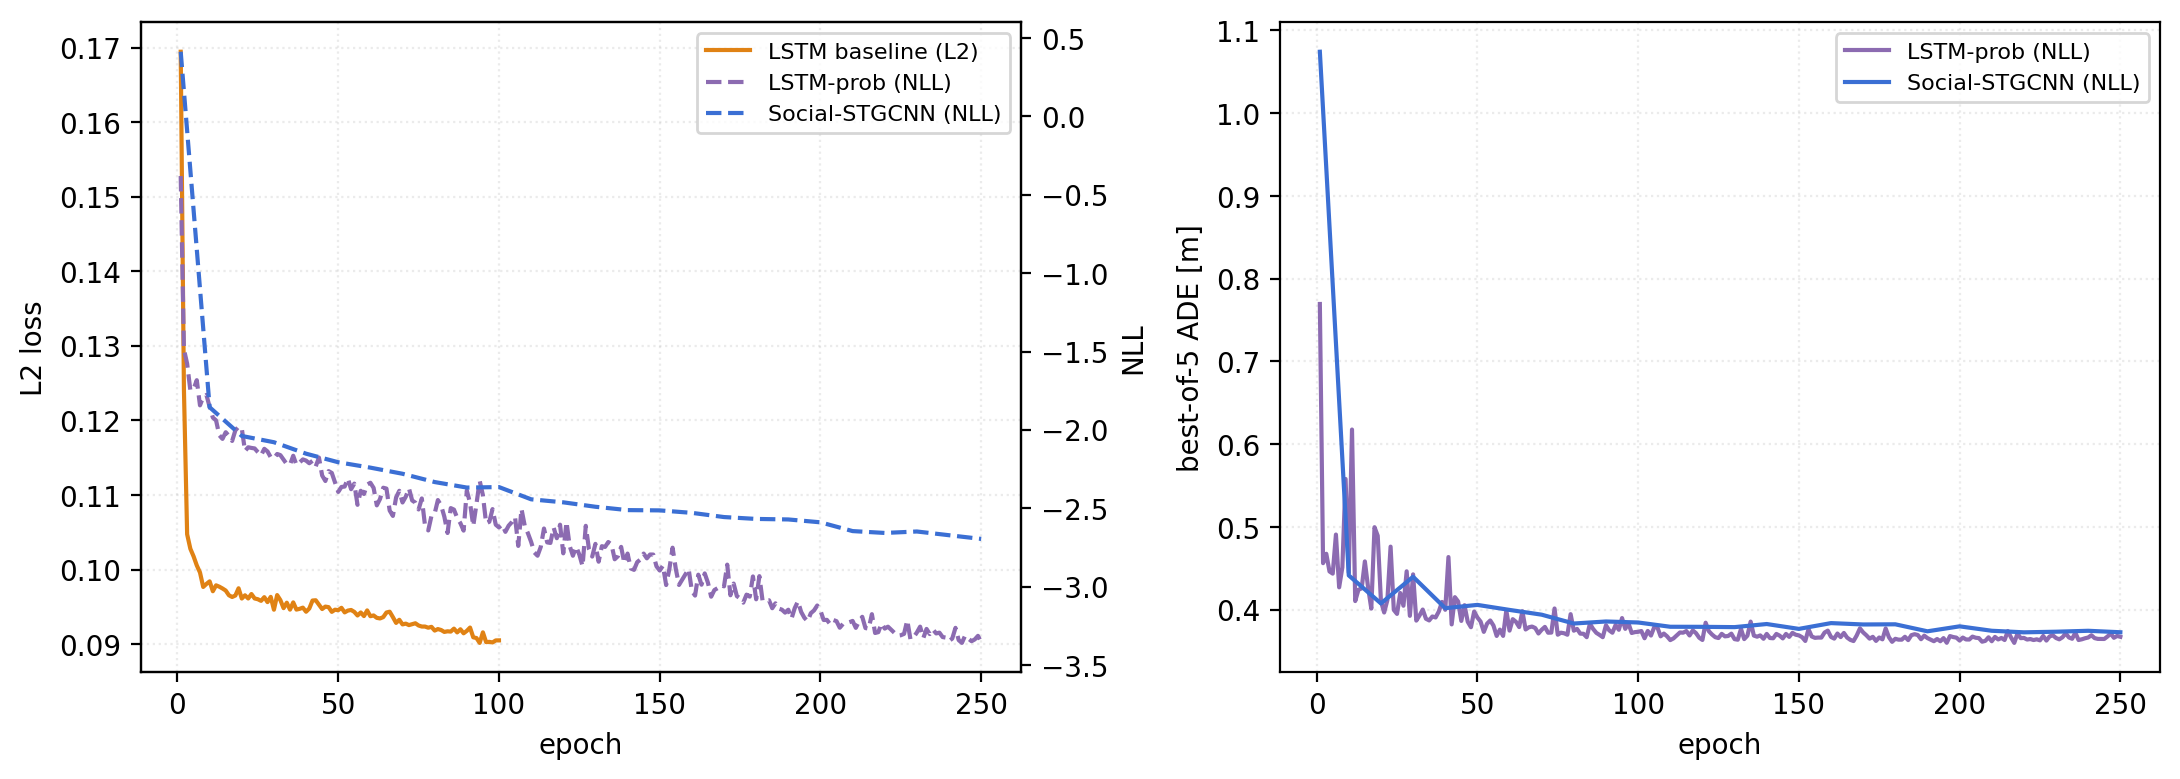
\includegraphics[width=\columnwidth]{figures/en/curves_zara1.png}
\caption{Training dynamics on ZARA1. Left: training losses; $L_2$ and NLL objectives are
plotted on separate axes as they are not on a common scale. Right: validation ADE for the
two probabilistic models under the identical best-of-5 protocol, the only mutually
comparable curves. They converge to indistinguishable error.}
\label{fig:curves}
\end{figure}

\subsection{Where the improvement actually comes from}

Two factors do produce substantial, measurable gains.

First, \textbf{uncertainty modeling}. Moving from a point prediction to a distribution
reduces average ADE from $0.552$~m to $0.405$~m, a $27\%$ improvement. This gain is
obtained by the interaction-agnostic architecture and is therefore unrelated to the graph.
The mechanism is multimodality: a model trained to emit a single point learns the
conditional expectation, which for a pedestrian approaching a junction lies between the
plausible outcomes, a location the pedestrian will never occupy.

Second, \textbf{parameter efficiency}. Social-STGCNN matches the LSTM using $7{,}563$
against $199{,}106$ parameters, a $26\times$ reduction (Table~\ref{tab:published}). For an
embedded robot controller with constrained memory and power budgets this is a substantive
practical advantage even at equal accuracy, and it is the strongest claim for the graph
architecture that our evidence supports.

\subsection{Hyperparameter optimization}

The TPE search over the graph model converged towards a wider temporal decoder
($n_{txpcnn}$ from $5$ to $7$), a larger temporal kernel ($3$ to $5$) and moderate dropout,
improving validation ADE from $0.419$ to $0.389$~m on ZARA1 over $15$ trials, $6$ of which
were pruned early. Notably the search did \emph{not} favour additional graph convolution
blocks, preferring deeper temporal processing, an independent signal consistent with our
main finding.

Retraining with the selected configuration yielded a test ADE of $0.283$~m, identical to
the default configuration ($0.283$~m), with FDE improving only from $0.498$ to $0.497$~m.
The validation gain therefore did not transfer to the test set. We report this rather than
omit it: it indicates the default architecture was already near the ceiling for this
dataset, and it illustrates why hyperparameters must be selected on validation and then
verified on held-out data.

\subsection{Qualitative analysis}

Fig.~\ref{fig:traj} compares predictions on a ZARA1 scene containing seven pedestrians.
Both models capture the dominant bidirectional flow; neither anticipates the mid-horizon
direction changes visible in the ground truth, and their predictions are largely
indistinguishable from one another, a visual counterpart to Table~\ref{tab:controlled}.

\begin{figure}[t]
\centering
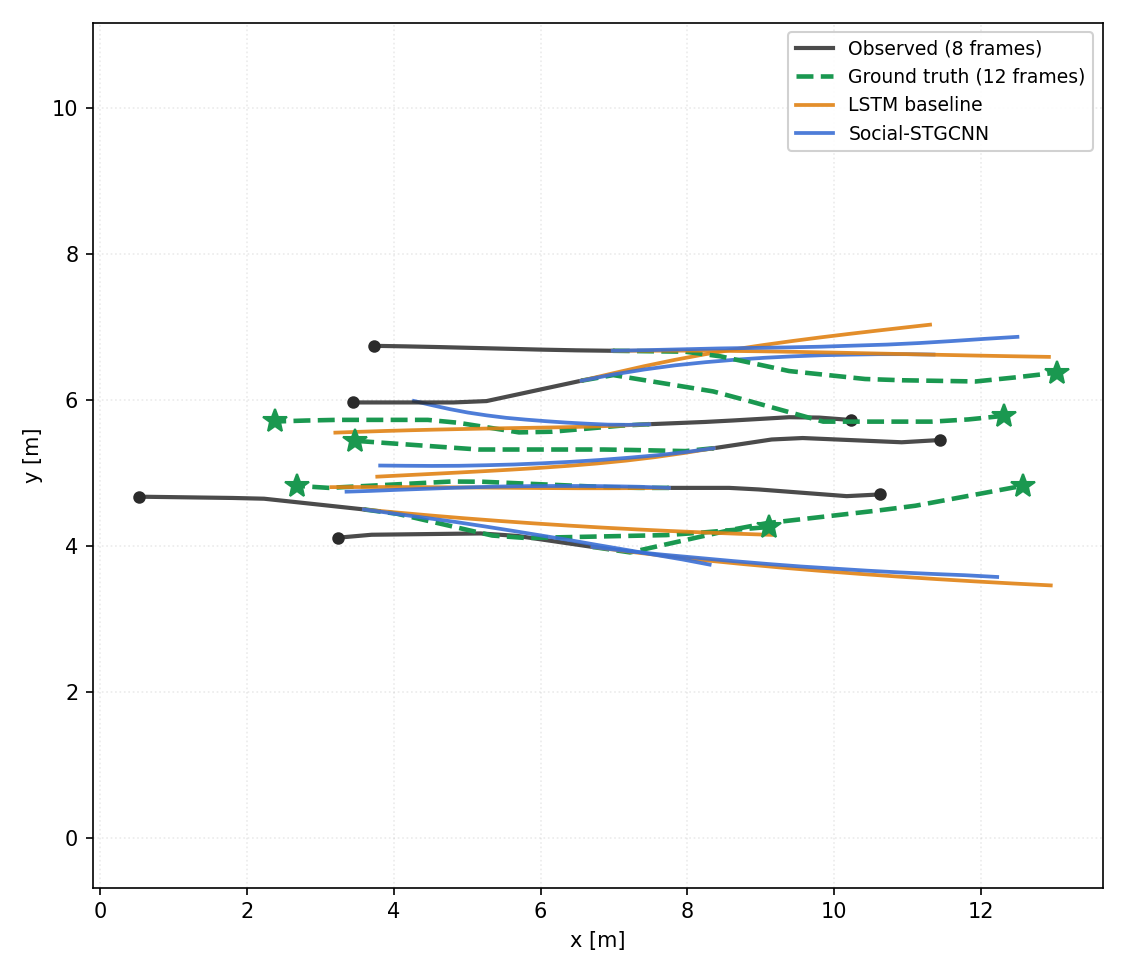
\includegraphics[width=\columnwidth]{figures/en/trajectories_zara1_00.png}
\caption{Qualitative comparison on ZARA1. Observed history (black), ground truth future
(green dashed), LSTM baseline (orange) and Social-STGCNN (blue). Stars mark the true final
positions.}
\label{fig:traj}
\end{figure}

Fig.~\ref{fig:heatmap} shows the predicted motion density, obtained by drawing $2{,}000
$ trajectories from the learned distribution. The density widens with the prediction
horizon, reflecting growing uncertainty, and separates into distinct lobes corresponding to
the two opposing pedestrian flows. This field is directly usable as a cost map by a
socially-aware planner, and it is the practical product of uncertainty modeling rather than
of the graph structure.

\begin{figure}[t]
\centering
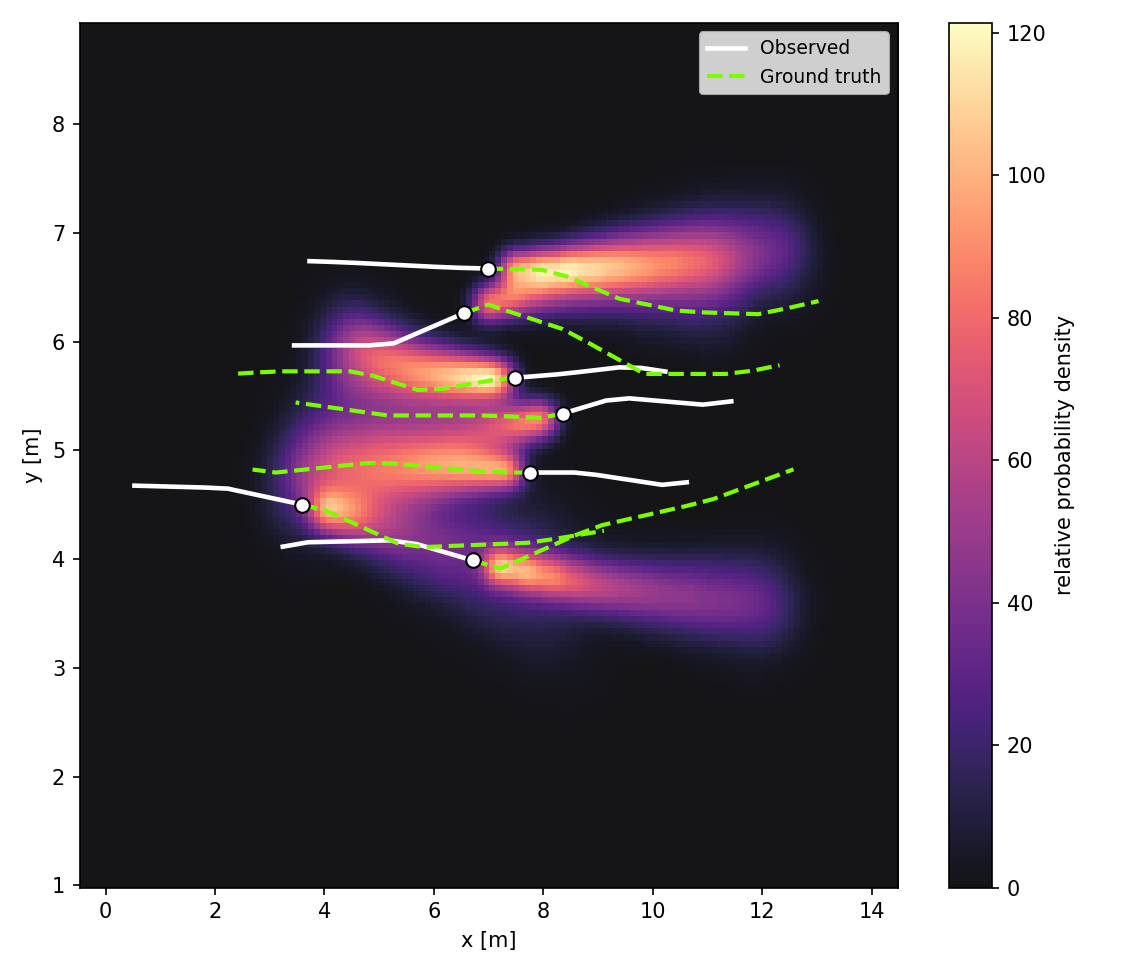
\includegraphics[width=\columnwidth]{figures/en/heatmap_zara1_00.png}
\caption{Predicted motion density on ZARA1 from $2{,}000$ samples of the learned
distribution. White: observed history; green dashed: ground truth. Uncertainty grows with
the horizon and separates by direction of travel.}
\label{fig:heatmap}
\end{figure}

\section{Discussion}

Our results indicate that on ETH-UCY, at a $4.8$~s horizon, explicit graph-based
interaction modeling does not improve average predictive accuracy relative to an
architecture that cannot observe other agents. Three considerations argue that this
reflects the benchmark rather than a defective implementation: both models reproduce
published performance; all models share a single data pipeline, so no difference can
originate from the data; and the loss, selection criterion and evaluation protocol are
identical between the two compared models.

The most plausible explanation is that pedestrian motion over this horizon is dominated by
inertia. People rarely change direction abruptly, both physically and because their
intention persists over several seconds. Most of the achievable error reduction therefore
comes from extrapolating current heading and speed accurately, not from reasoning about
interaction. This is consistent with~\cite{scholler2020constant}, who reach a related
conclusion using a constant velocity model. Situations in which interaction is decisive
(last-moment collision avoidance, circumventing a group) are a small fraction of windows,
so a model that handles them perfectly gains little in the average.

The single scene on which the graph model wins clearly, HOTEL, is consistent with this
account. HOTEL contains many stationary or slowly-moving people near an entrance, precisely
the regime in which "continue straight" is weakest and contextual information about
neighbours is most informative. The graph helps where inertia does not.

For socially-aware navigation the implication is a refinement rather than a rejection of
the original premise. What a planner most needs is a calibrated distribution over future
positions, such as that in Fig.~\ref{fig:heatmap}, and this is supplied by either
architecture. Where the graph model retains a decisive advantage is deployment cost:
equivalent accuracy at $26\times$ fewer parameters.

\section{Limitations and Future Work}

The models consume no map of the environment and will therefore predict trajectories
through walls when the current heading points that way. Groups are not modeled explicitly.
Perfect detection and tracking are assumed, whereas a deployed robot receives noisy
detections with identity switches. The best-of-$20$ protocol is optimistic: a robot must
act on a single belief rather than select the most fortunate of twenty samples. Finally,
the hyperparameter search was conducted on a single scene, and the step from prediction to
socially-aware planning is not implemented.

The most direct test of our interpretation would extend the prediction horizon beyond
$8$--$10$~s, where inertia should cease to dominate and interaction modeling would be
expected to show a clearer advantage. Adding a semantic map would eliminate physically
impossible predictions, and integrating the predicted density into a local planner would
allow the practical value of the distribution to be measured directly.

\section{Conclusion}

We examined whether explicit social interaction modeling improves pedestrian trajectory
prediction, using a comparison controlled for training objective and evaluation protocol.
On ETH-UCY at a $4.8$~s horizon it does not: a graph-based model attains $0.415$~m ADE
against $0.405$~m for an architecture that never observes other pedestrians. The
improvements that are real lie elsewhere: uncertainty modeling reduces error by $27\%$,
and the graph architecture achieves equivalent accuracy with $26\times$ fewer parameters.
We conclude that for socially-aware navigation the valuable output is a calibrated
distribution over future positions, and that claims about the benefit of interaction
modeling should be substantiated with comparisons in which the training objective is held
fixed.

\section*{Reproducibility}

The complete implementation, trained checkpoints, hyperparameter search logs and the
scripts that generate every table and figure in this paper are available in the project
repository.

\bibliographystyle{IEEEtran}
\bibliography{refs}

\end{document}
